\section{Технический проект}
\subsection{Общая характеристика организации решения задачи}

Необходимо спроектировать и разработать веб-приложение, направленное на поддержку самостоятельного изучения JavaScript иностранными студентами. Платформа представляет собой совокупность взаимосвязанных веб-сервисов, доступных через единый пользовательский интерфейс, реализованный с использованием современных веб-технологий: HTML, CSS, JavaScript и Python (Django).

Каждый сервис (модуль) обеспечивает выполнение образовательных задач: управление курсами, уроками, тестами, результатами и локализацией. Платформа размещается в сети Интернет по определённому доменному имени (например, https://swsueducate.ru). Интерфейс реализован с использованием фреймворка Bootstrap для адаптивности, а клиентская интерактивность обеспечивается через JavaScript (например, Sortable.js для сортировки уроков). Серверная часть, построенная на Django, обрабатывает запросы, управляет данными и генерирует динамические страницы.

\subsection{Обоснование выбора технологии проектирования}

На сегодняшний день информационный рынок, поставляющий программные решения в выбранной сфере, предлагает множество продуктов, позволяющих достигнуть поставленной цели – разработки веб-платформы.

\subsubsection{Описание используемых технологий и языков программирования}

В процессе разработки веб-платформы используются программные средства и языки программирования. Каждое программное средство и каждый язык программирования применяется для круга задач, при решении которых они необходимы.

\subsubsection{Язык программирования Python}

Python — это высокоуровневый язык программирования общего назначения с поддержкой нескольких парадигм, включая объектно-ориентированное, процедурное и функциональное программирование. Благодаря своей простоте, читаемости и обширной экосистеме библиотек, Python широко применяется в разработке веб-приложений, автоматизации процессов, анализе данных, машинном обучении и многих других областях. В контексте разработки веб-приложений Python используется совместно с фреймворками, такими как Django и Flask, которые обеспечивают удобные средства для создания серверной логики, обработки запросов и генерации динамических веб-страниц.

\subsubsection{Язык программирования JavaScript}

\paragraph{Достоинства языка JavaScript}

JavaScript — это высокоуровневый интерпретируемый язык программирования, основной задачей которого является создание интерактивного поведения на веб-страницах. Он является неотъемлемой частью технологии разработки клиентской части веб-приложений и поддерживается всеми современными веб-браузерами. С помощью JavaScript можно реализовывать динамическое обновление содержимого, проверку данных на стороне клиента, обработку событий, а также взаимодействие с сервером без перезагрузки страницы (через AJAX-запросы). Современные стандарты JavaScript (начиная с ECMAScript 6) предоставляют широкий набор возможностей, включая модули, асинхронные функции, классы и работу с промисами. Для повышения совместимости и ускорения разработки часто используются библиотеки и фреймворки, такие как jQuery, React, Vue.js и другие. Они позволяют упростить доступ к элементам DOM, реализовать реактивные интерфейсы и обеспечить кроссбраузерную поддержку. JavaScript выполняется непосредственно в браузере пользователя, что позволяет создавать отзывчивые и интерактивные пользовательские интерфейсы без необходимости постоянной связи с сервером.

\paragraph{Недостатки языка JavaScript}

\begin{itemize}
  \item parseInt("08") // → 0
  \item parseInt("0x10") // → 16
  \item parseInt("0x10", 10) // → 0
  \item null == 0 // → false
  \item null > 0 // → false
  \item null >= 0 // → true
  \item undefined == null // → true
  \item undefined === null // → false
  \item typeof NaN // → "number"
  \item NaN === NaN // → false
  \item "5" + 3 // → "53"
  \item "5" - 3 // → 2
  \item "5" * "3" // → 15
  \item "5" * "abc" // → NaN
  \item 0.1 + 0.2 === 0.3 // → false
  \item (0.1 + 0.2).toFixed(1) // → "0.3"
  \item true + true // → 2
  \item true - false // → 1
  \item "1" + true // → "1true"
  \item "1" - true // → 0
\end{itemize}



\subsection{Структура базы данных}

Проанализировав требования, можно выделить следующие основные сущности:

\begin{itemize}
	\item "<Курсы">;
	\item "<Уроки">;
	\item "<Тесты">;
	\item "<Результаты тестов">;
	\item "<Пользователи">;
	\item "<Локализация">;
	\item "<Уведомления">;
	\item "<Панель управления">.
\end{itemize}

Отношение между таблицами базы данных отражены на (рис.~\ref{bd:image})

\begin{figure}[ht]
	\center{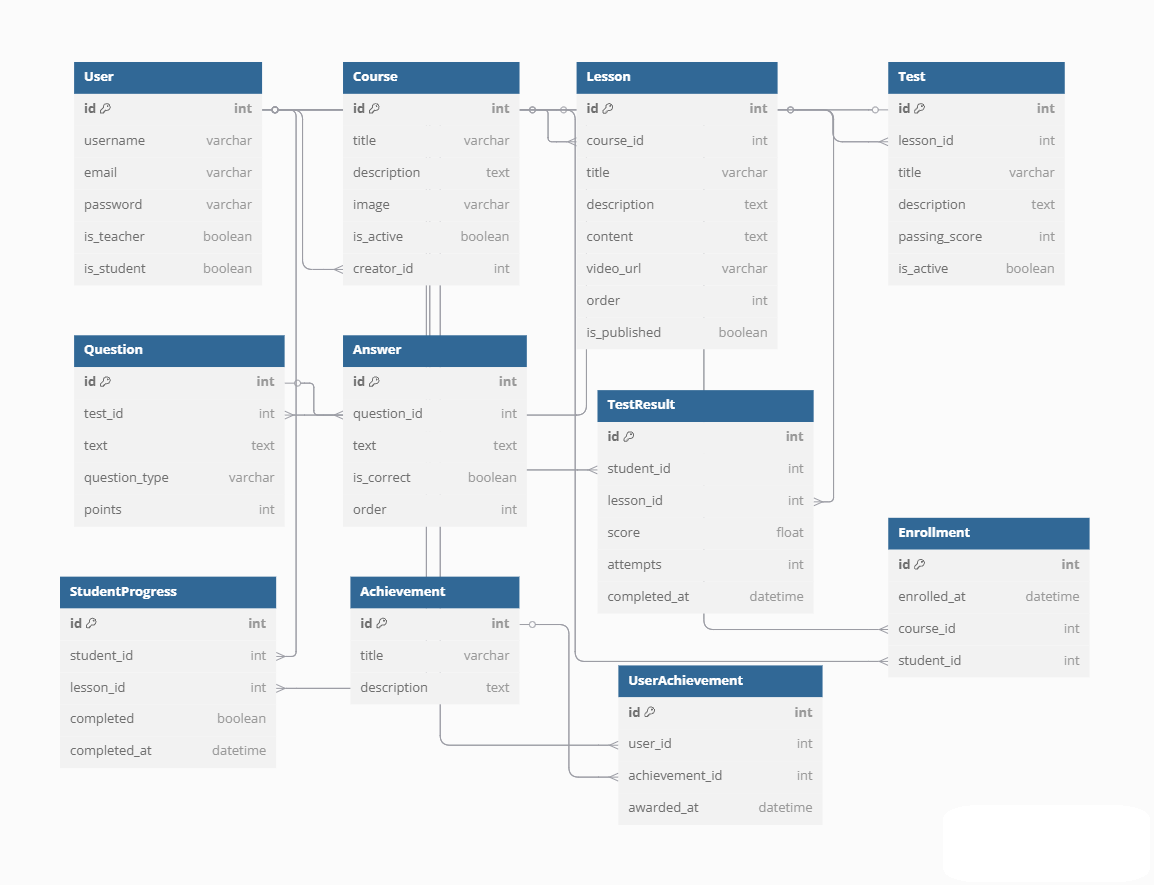
\includegraphics[width=1\linewidth]{images/бд}}
	\caption{Структура базы данных}
	\label{bd:image}
\end{figure}

В состав сущностей входят следующие атрибуты:

\begin{xltabular}{\textwidth}{|l|l|p{3.2cm}|X|}
	\caption{Атрибуты сущности <<Курсы>>\label{courses:table}}\\ \hline
	Поле & Тип & Обязательное & Описание \\ \hline
	\endfirsthead
	\continuecaption{Продолжение таблицы \ref{courses:table}}\\ \hline
	Поле & Тип & Обязательное & Описание \\ \hline
	\endhead
	id & Integer & true & Уникальный идентификатор курса \\ \hline
	title & String & true & Название курса \\ \hline
	description & Text & true & Описание курса \\ \hline
	image & String & false & Путь к изображению курса \\ \hline
	isactive & Boolean & true & Признак активности курса \\ \hline
	createdat & DateTime & true & Дата создания курса \\ \hline
	teacherid & ForeignKey & true & Преподаватель (ссылка на таблицу Пользователи) \\ \hline
\end{xltabular}

\begin{xltabular}{\textwidth}{|l|l|p{3.2cm}|X|}
	\caption{Атрибуты сущности <<Уроки>>\label{lessons:table}}\\ \hline
	Поле & Тип & Обязательное & Описание \\ \hline
	\endfirsthead
	\continuecaption{Продолжение таблицы \ref{lessons:table}}\\ \hline
	Поле & Тип & Обязательное & Описание \\ \hline
	\endhead
	id & Integer & true & Уникальный идентификатор урока \\ \hline
	courseid & ForeignKey & true & Курс, к которому относится урок (ссылка на таблицу Курсы) \\ \hline
	title & String & true & Название урока \\ \hline
	description & Text & false & Описание урока \\ \hline
	content & Text & true & Содержимое урока (текст, HTML) \\ \hline
	videourl & String & true & Ссылка на видео урока \\ \hline
	order & Integer & true & Порядок урока в курсе \\ \hline
	ispublished & Boolean & true & Признак публикации урока \\ \hline
	createdat & DateTime & true & Дата создания урока \\ \hline
\end{xltabular}

\begin{xltabular}{\textwidth}{|l|l|p{3.2cm}|X|}
	\caption{Атрибуты сущности <<Тесты>>\label{tests:table}}\\ \hline
	Поле & Тип & Обязательное & Описание \\ \hline
	\endfirsthead
	\continuecaption{Продолжение таблицы \ref{tests:table}}\\ \hline
	Поле & Тип & Обязательное & Описание \\ \hline
	\endhead
	id & Integer & true & Уникальный идентификатор теста \\ \hline
	lessonid & ForeignKey & true & Урок, к которому относится тест (ссылка на таблицу Уроки) \\ \hline
	title & String & true & Название теста \\ \hline
	description & Text & true & Описание теста \\ \hline
	isactive & Boolean & true & Признак активности теста \\ \hline
	passingscore & Integer & true & Проходной балл (в процентах) \\ \hline
	createdat & DateTime & false & Дата создания теста (может отсутствовать) \\ \hline
\end{xltabular}

\begin{xltabular}{\textwidth}{|l|l|p{3.2cm}|X|}
	\caption{Атрибуты сущности <<Тесты>>\label{tests:table}}\\ \hline
	Поле & Тип & Обязательное & Описание \\ \hline
	\endfirsthead
	\continuecaption{Продолжение таблицы \ref{tests:table}}\\ \hline
	Поле & Тип & Обязательное & Описание \\ \hline
	\endhead
	id & Integer & true & Уникальный идентификатор теста \\ \hline
	lesson & ForeignKey & true & Урок, к которому относится тест \\ \hline
	title & String & true & Название теста \\ \hline
	questions & Array & false & Список вопросов (JSON или связанные модели) \\ \hline
	createdAt & DateTime & true & Дата создания \\ \hline
\end{xltabular}

\begin{xltabular}{\textwidth}{|l|l|p{3.2cm}|X|}
	\caption{Атрибуты сущности <<Результаты тестов>>\label{test_results:table}}\\ \hline
	Поле & Тип & Обязательное & Описание \\ \hline
	\endfirsthead
	\continuecaption{Продолжение таблицы \ref{test_results:table}}\\ \hline
	Поле & Тип & Обязательное & Описание \\ \hline
	\endhead
	id & Integer & true & Уникальный идентификатор результата \\ \hline
	studentid & ForeignKey & true & Студент (ссылка на таблицу Пользователи) \\ \hline
	lessonid & ForeignKey & true & Урок, связанный с тестом (ссылка на таблицу Уроки) \\ \hline
	score & Float & true & Оценка (в процентах или дробное значение) \\ \hline
	attempts & Integer & true & Количество попыток \\ \hline
	answers & Text & true & Ответы (в формате JSON) \\ \hline
	completedat & DateTime & true & Дата завершения теста \\ \hline
\end{xltabular}

\begin{xltabular}{\textwidth}{|l|l|p{3.2cm}|X|}
	\caption{Атрибуты сущности <<Пользователи>>\label{users:table}}\\ \hline
	Поле & Тип & Обязательное & Описание \\ \hline
	\endfirsthead
	\continuecaption{Продолжение таблицы \ref{users:table}}\\ \hline
	Поле & Тип & Обязательное & Описание \\ \hline
	\endhead
	id & Integer & true & Уникальный идентификатор пользователя \\ \hline
	username & String & true & Имя пользователя \\ \hline
	email & String & true & Электронная почта \\ \hline
	isteacher & Boolean & true & Признак преподавателя \\ \hline
	password & String & true & Хэшированный пароль пользователя \\ \hline
	lastlogin & DateTime & false & Дата последнего входа \\ \hline
	issuperuser & Boolean & true & Признак суперпользователя \\ \hline
	firstname & String & true & Имя пользователя \\ \hline
	lastname & String & true & Фамилия пользователя \\ \hline
	isstaff & Boolean & true & Признак персонала \\ \hline
	isactive & Boolean & true & Признак активности пользователя \\ \hline
	datejoined & DateTime & true & Дата регистрации \\ \hline
	isstudent & Boolean & true & Признак студента \\ \hline
	isadmin & Boolean & true & Признак администратора \\ \hline
\end{xltabular}

\begin{xltabular}{\textwidth}{|l|l|p{3.2cm}|X|}
	\caption{Атрибуты сущности <<Запись на курсы>>\label{enrollments:table}}\\ \hline
	Поле & Тип & Обязательное & Описание \\ \hline
	\endfirsthead
	\continuecaption{Продолжение таблицы \ref{enrollments:table}}\\ \hline
	Поле & Тип & Обязательное & Описание \\ \hline
	\endhead
	id & Integer & true & Уникальный идентификатор записи \\ \hline
	enrolledat & DateTime & true & Дата записи на курс \\ \hline
	courseid & ForeignKey & true & Курс (ссылка на таблицу Курсы) \\ \hline
	studentid & ForeignKey & true & Студент (ссылка на таблицу Пользователи) \\ \hline
\end{xltabular}

\begin{xltabular}{\textwidth}{|l|l|p{3.2cm}|X|}
	\caption{Атрибуты сущности <<Прогресс>>\label{progress:table}}\\ \hline
	Поле & Тип & Обязательное & Описание \\ \hline
	\endfirsthead
	\continuecaption{Продолжение таблицы \ref{progress:table}}\\ \hline
	Поле & Тип & Обязательное & Описание \\ \hline
	\endhead
	id & Integer & true & Уникальный идентификатор прогресса \\ \hline
	completed & Boolean & true & Признак завершения урока \\ \hline
	completedat & DateTime & false & Дата завершения урока \\ \hline
	lessonid & ForeignKey & true & Урок (ссылка на таблицу Уроки) \\ \hline
	studentid & ForeignKey & true & Студент (ссылка на таблицу Пользователи) \\ \hline
\end{xltabular}

\begin{xltabular}{\textwidth}{|l|l|p{3.2cm}|X|}
	\caption{Атрибуты сущности <<Вопросы>>\label{questions:table}}\\ \hline
	Поле & Тип & Обязательное & Описание \\ \hline
	\endfirsthead
	\continuecaption{Продолжение таблицы \ref{questions:table}}\\ \hline
	Поле & Тип & Обязательное & Описание \\ \hline
	\endhead
	id & Integer & true & Уникальный идентификатор вопроса \\ \hline
	testid & ForeignKey & true & Тест (ссылка на таблицу Тесты) \\ \hline
	text & Text & true & Текст вопроса \\ \hline
	questiontype & String & true & Тип вопроса (например, выбор, текст) \\ \hline
	points & Integer & true & Баллы за вопрос \\ \hline
\end{xltabular}

\begin{xltabular}{\textwidth}{|l|l|p{3.2cm}|X|}
	\caption{Атрибуты сущности <<Ответы>>\label{answers:table}}\\ \hline
	Поле & Тип & Обязательное & Описание \\ \hline
	\endfirsthead
	\continuecaption{Продолжение таблицы \ref{answers:table}}\\ \hline
	Поле & Тип & Обязательное & Описание \\ \hline
	\endhead
	id & Integer & true & Уникальный идентификатор ответа \\ \hline
	questionid & ForeignKey & true & Вопрос (ссылка на таблицу Вопросы) \\ \hline
	text & Text & true & Текст ответа \\ \hline
	iscorrect & Boolean & true & Признак правильности ответа \\ \hline
	order & Integer & true & Порядок ответа \\ \hline
\end{xltabular}

\begin{xltabular}{\textwidth}{|l|l|p{3.2cm}|X|}
	\caption{Атрибуты сущности <<Связь пользователей и курсов>>\label{user_courses:table}}\\ \hline
	Поле & Тип & Обязательное & Описание \\ \hline
	\endfirsthead
	\continuecaption{Продолжение таблицы \ref{user_courses:table}}\\ \hline
	Поле & Тип & Обязательное & Описание \\ \hline
	\endhead
	id & Integer & true & Уникальный идентификатор записи \\ \hline
	userid & ForeignKey & true & Пользователь (ссылка на таблицу Пользователи) \\ \hline
	courseid & ForeignKey & true & Курс (ссылка на таблицу Курсы) \\ \hline
\end{xltabular}

Экземпляры этих сущностей реализуются в информационных блоках пользовательского интерфейса. Атрибуты сущностей отображаются в полях, свойствах и компонентах соответствующих элементов.


\subsection{Диаграмма компонентов}

Диаграмма компонентов (рис.~\ref{diag:image}) отображает взаимодействие пользователей (студентов и преподавателей) с сервисами платформы. Она помогает определить архитектуру, показывая связи между компонентами, включая клиентскую часть и серверную часть. Основными элементами диаграммы являются компоненты (например, курсы), их интерфейсы и зависимости между ними.


\begin{figure}[htp!]
	\centering{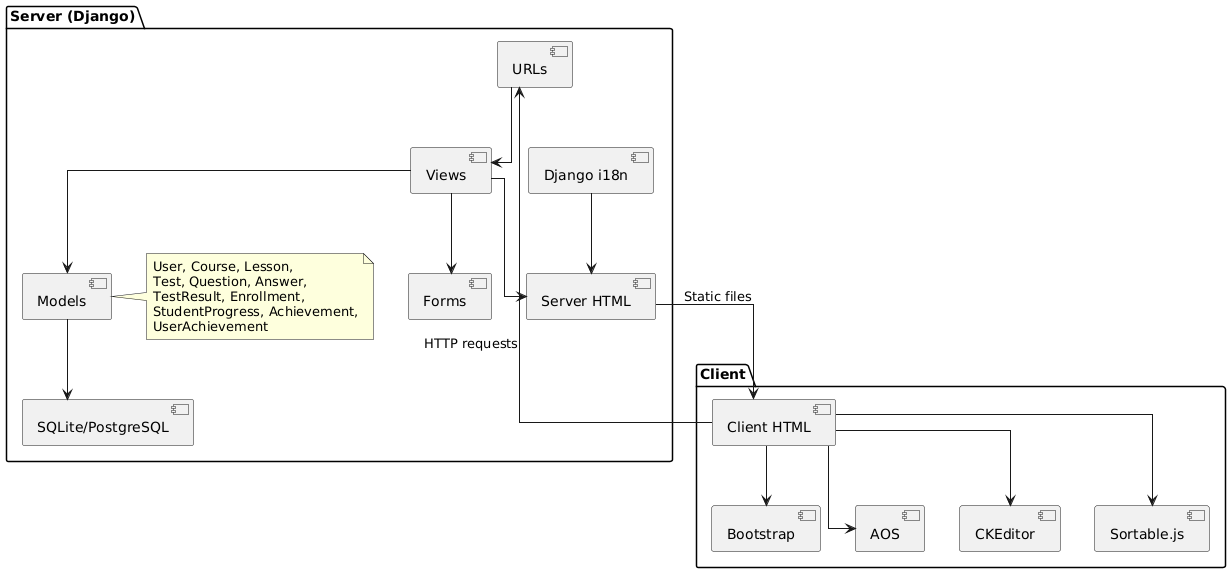
\includegraphics[width=0.7\linewidth]{images/диаграмма1}}
	\caption{Диаграмма компонентов}
	\label{diag:image}
\end{figure}

